\subsection{Reconocimiento de caracteres}
\label{subsection: wang_recon_caracteres}
	
	El reconocimiento de caracteres, es la primera etapa en el pipeline de procesamiento que desarrollaron Wang et al. Dada una imagen, inicialmente es necesario detectar las potenciales ubicaciones de los caracteres dentro de la misma. Para lograr esto, los autores realizan una detección a múltiple escala usando un algoritmo de clasificación de ventana deslizante. Esta ventana al comienzo tiene un tamaño fijo y  recorre la imagen detectando potenciales caracteres dentro de sí. Luego aumenta su tamaño con el objetivo de poder detectar caracteres más grandes. Supongamos que la ventana está ubicada en una zona de la imagen donde hay un caracter a detectar. Si quisieramos reconocer ese caracter, sería necesario compararlo con los 62 posibles caracteres existentes. Dado que hay muchas clases involucradas, los autores tienen que lograr clasificar cada nueva entrada dentro de las 62 posibles clases. Estas clases estan formadas por los caracteres alfabéticos (en minúscula y mayúscula, 52 en total) y numéricos (10 en total). La solución adoptada por los autores es usar \textit{random ferns} (ver subsección \ref{subsection:ferns}) como su clasificador. Esto se debe a que es un clasificador eficiente y puede manejar múltiples clases.
	
	Para entrenar a este clasificador, los autores realizan dos pruebas diferentes. La primera consta de entrenar al clasificador con imágenes recortadas de caracteres que obtuvieron del dataset público \textit{Chars74k}. Este dataset consta de aproximadamente 15 imágenes naturales por clase para el entrenamiento y 15 imágenes por clase para la evaluación. La segunda prueba la realizan sobre datos sintéticos creados por ellos mismos. Dada la gran variabilidad de apariencias que hay en las imágenes reales y a lo difícil que es recolectar un conjunto de este tipo, es que surge esta segunda prueba. Esto supone una gran ventaja por la cantidad ilimitada de datos que se puede manejar. Este enfoque fue aprovechado por los autores, que sintetizaron alrededor de 1000 imágenes por carácter usando 40 fuentes. El objetivo de esto era obtener imágenes de caracteres que se asemejaran a las imágenes reales. Para lograr esto, a cada imagen de fuente le aplicaban una serie de transformaciones que alteraban su aspecto en un intento de imitar los diferentes aspectos que podía tener una imagen natural. Como se puede observar en la Figura \ref{fig: Datos sinteticos Wang}, estas imágenes tienen variaciones en el color de la letra y el fondo, como así también la inclinación del carácter y su posición dentro de la imagen.
	
		\begin{figure}[htbp]
			\centering
			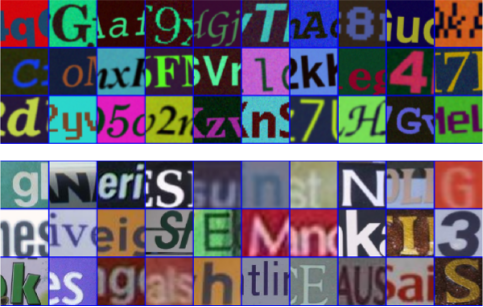
\includegraphics[scale=0.5]{img/synth_data_wang.png}
			\caption[Datos sintéticos Wang]{Arriba se puede ver el conjunto de imágenes sintéticas creadas por Wang et. al. Estas imágenes tienen una dimensión de 48x48 píxeles e intentan imitar a las imágenes reales. Abajo se puede observar un conjunto de imágenes reales recortadas que  fueron extraidas del dataset ICDAR. La figura fue extraida del trabajo de Wang et. al. \cite{wang}.}
			\label{fig: Datos sinteticos Wang}
		\end{figure}
	
	Para poder reconocer un símbolo, se tienen que extrear aquellas características que lo distingue de otros símbolos (sección \ref{subsection:feature}), es decir, aquello que lo hace único. En particular, una forma de lograr esto es a traves de los gradientes de la imagen (ver \ref{subsubsection: Gradientes}). Para poder aprovecharse de esto, Wang et. al. hacen uso del descriptor de características HOG (ver \ref{subsection:hog}). Estos descriptores han demostrado ser útiles en tareas de clasificación \cite{DT05}. Luego, para el entrenamiento de \textit{Random Ferns}, se tienen los descriptores HOG de cada imagen para cada una de las 62 clases. Sin embargo, no es suficiente para poder empezar a entrenar ya que \textit{Random Ferns} hace uso de descriptores binarios (ver sección \ref{subsection:hog}) para la clasificación pues son fáciles de computar, almacenar y escala con la cantidad de clases. En su trabajo, especifican que los vectores binarios consisten en la aplicación de umbrales elegidos aleatoriamente sobre entradas elegidas al azar del vector HOG. Un vez binarizados los descriptores es posible entrenar al clasificador y dejarlo listo para clasificar nuevas instancias de imágenes de caracteres.
	
	El pipeline de reconocimiento sigue, un vez que se ha detectado un caracter, con una técnica denominada \textit{supresión de los máximos} (\textit{NMS} por sus siglas en inglés). Esta técnica se aplica sobre el caracter detectado y es una técnica muy usada en los algoritmos de visión por computadora. Básicamente, suprime los píxeles en la imagen que no son máximos locales (con respecto a los píxeles vecinos) a lo largo de la dirección del gradiente. \RC{Faltaria agregar algo mas sobre NMS}. Con esto los autores dan por finalizada la etapa de reconocimiento de caracteres.


